\chapter{Theoretische Grundlagen}\label{sec:grundlagen}

In diesem Kapitel werden die für diese Arbeit besonders wichtigen theoretischen Grundlagen dargelegt. 
Diese sind vorallem Vorüberlegungen zur Geometrie und elektronischen Eigenschaften des Bienenwabengitters, sowie die wichtigsten Punkte der konventiellen Theorie zu Supraleitung, der BCS-Theorie.

\section{Bienenwabengitter}

Das Bienenwabengitter ist eine zweidimensionale Gitterstruktur, deren Elemente in einem hexagonalen Muster angeordnet sind. 
Ein prominentes Beispiel für ein Material mit Bienenwabenstruktur ist das kohlenstoffbasierte \textit{Graphen}~\cite{castro_neto_electronic_2009} bzw. die Monolayer des Graphits, aber  auch in Übergangsmetall-Dichalkogeniden (TMDs) wie \textit{MoS2} oder \textit{MoSe2} kommt diese Struktur vor. \\
Das Gitter selbst muss im Gegensatz zu einem einfachen hexagonalen Gitter durch gegeneinander verschobene Untergitter $A$ und $B$ beschrieben werden, die jeweils eine hexagonale Struktur aufweisen, siehe Abbildung \autoref{fig:gitter}.
\begin{figure}[htbp]
    \centering
    
\includegraphics[width=0.4\textwidth]{images/gitter.png}
    \caption{Skizze des Bienenwabengitters mit den Untergittern $A$ und $B$. Ebenfalls zu sehen sind die primitiven Gittervektoren $\vec{a}_1$ und $\vec{a}_2$, sowie die nearest-neighbor Vektoren $\vd{1}$, $\vd{2}$ und $\vd{3}$~\cite{castro_neto_electronic_2009}.}
    \label{fig:gitter}
\end{figure}

Die Untergitter $A$ und $B$ besitzen dieselben primitiven Gittervektoren, sind jedoch um einen der drei Nearest-Neighbour-Vektoren $\vdelta_1$, $\vdelta_2$ und $\vdelta_3$ 
\begin{align}
    \vd{1} &= \frac{a}{2} \begin{pmatrix}1 \\ \sqrt{3}\end{pmatrix} & \vd{2} &= \frac{a}{2} \begin{pmatrix}1 \\ -\sqrt{3}\end{pmatrix} & \vd{3} &= a \begin{pmatrix}-1 \\ 0\end{pmatrix}
    \label{eq:nn-vektoren}
\end{align}
zueinander verschoben, wobei $a$ den Gitterabstand bezeichnet. 
Da die Nearest-Neighbour-Vektoren nicht als ganzzahlige lineare Kombination der primitiven Gittervektoren $\vec{a_1}$ und $\vec{a_2}$
\begin{align}
    \vec{a_1} &= \frac{a}{2} \begin{pmatrix}3 \\ \sqrt{3}\end{pmatrix} & \vec{a_2} &= \frac{a}{2} \begin{pmatrix}-3 \\ \sqrt{3}\end{pmatrix}
\end{align}
dargestellt werden können, muss das Bienenwabengitter also mit einer zweiatomigen Basis aus den Untergittern $A$ und $B$ beschrieben werden.\\
Als quantenmechanische Beschreibung der elektronischen Struktur des Gitters wird ein Tight-Binding-Modell (TB) verwendet. 
Dabei wird angenommen, dass Elektronen stark an ihr zugehöriges Gitteratom gebunden werden, da dessen Atomorbitale nur schwach mit den Orbitalen benachbarter Atome überlappen. 
Die Elektronen sind also in einem Gitterplatz lokalisiert, können jedoch mit einer bestimmten Wahrscheinlichkeit zu einem anderen Gitterplatz tunneln (\glqq hopping \grqq)~\cite{ashcroft_solid_1976}. 
Der verwendete Tight-Binding-Hamiltonoperator lautet
\begin{align}
    \oH_\text{TB} &= -t \sum_{\expval{\vec{R}, \vec{R'}}, \sigma} \ofed{\vec{R}, \sigma} \ofe{\vec{R'}, \sigma} \label{eq:TB}\, ,
\end{align}
wobei hier nur ein Elektronorbital und Nearest-Neighbour-Hopping-Terme berücksichtigt werden, mit $\expval{\vec{R}, \vec{R'}}$ ist die Summe über alle möglichen Gittervektoren $\vec{R}$ und jeweiligen Nachbarn $\vec{R'}$ gemeint. $t$ ist die in einer Energie-Einheit gemessene Hopping-Wahrscheinlichkeit und $\ofed{\vec{R}, \sigma}$ und $\ofe{\vec{R'}, \sigma}$ sind die in der zweiten Quantisierung formulierten Erzeugungs- und Vernichtungsoperatoren für Elektronen mit Spin $\sigma$ an den Gitterplätzen $\vec{R}$ bzw. $\vec{R'}$.
Die fermionischen Operatoren erfüllen die Antikommutatorrelationen
\begin{align}
    \anticommute{\ofe{\alpha}}{\ofed{\beta}} &= \delta_{\alpha \beta} & \text{und} & &
    \anticommute{\ofe{\alpha}}{\ofe{\beta}} = \anticommute{\ofed{\alpha}}{\ofed{\beta}} &= 0 \label{eq:anticommute}\, ,
\end{align}
mit $\anticommute{\op{A}}{\op{B}} = \op{A} \op{B} + \op{B} \op{A}$.

% \red{\textbf{IDEEN: Noch etwas zur Brillouin-Zone schreiben bzw. primtive Vektoren und reziproke. Ist noch allgemein zu Bienenwabengitter, aber sowas wie DOS ist schon graphen-spezifisch, sowie das Modell eigentlich..}}

\section{BCS-Theorie}

Die gängigste Theorie zur Beschreibung von konventionellen Niedrigtemperatur-Supraleitern ist die von Bardeen, Cooper und Schrieffer (1957) entwickelte BCS-Theorie~\cite{bardeen_theory_1957,tinkham_introduction_2004}. 
Das folgenden Kapitel soll hierbei eine Einführung in die Grundkonzepte, die Limitierung, sowie der hier verwendeten Darstellung der BCS-Theorie geben. 

\subsection{Cooper-Paare}

Der Schlüsselmechanismus bei der Ausbildung einer supraleitenden Phase ist eine attraktive Wechselwirkung zweier Elektronen, die die Bildung eines neuen gebundenen Zustands, nämlich der sogenannten Cooper-Paare ermöglicht. 
Aufgrund ihres ganzzahligen Gesamtspins besitzen Cooper-Paare bosonischen Charakter und können unterhalb einer kritischen Temperatur einen gemeinsamen makroskopisch kohärenten Quantenzustand ausbilden.
Dieser wird durch den komplexen Ordnungsparameter $\Delta$ beschrieben, dessen Betrag im Rahmen der BCS-Theorie gleichzeitig die Energielücke für die Anregung eines einzelnes Quasiteilchens aus dem kondensierten Grundzustand bestimmt (vgl. Abschnitt~\ref{sec:modell}).
Es lässt sich zeigen, dass dieser makroskopische Quantenzustand genau die Eigenschaften einer supraleitenden Phase erfüllt, siehe dazu z.\,B. Ref.~\cite{tinkham_introduction_2004}.


\subsection{Phononenvermittelte Elektron-Elektron-Wechselwirkung}
Die Ursache der attraktiven Wechselwirkung mag aufgrund der Coulomb-Abstoßung zwischen den Elektronen zunächst kontraintuitiv erscheinen, kann in der BCS-Theorie aber durch die Kopplung der Elektronen mit den Phononen des Kristallgitters begründet werden. \\

Anschaulich lässt sich dies anhand der unterschiedlichen Zeitskalen für Gitterschwingungen und Elektronenbewegungen in Metallen erklären.
Regt ein Leitungselektron eine Gitterschwingung an, bewegt es sich in der Zeit, in der die ausgelenkten Atomrümpfe zurückschwingen um ein Vielfaches der Gitterkonstante weiter, während die zurückschwingenden Atomrümpfe selbst ein weiteres Elektron anziehen können. 
Es kommt also in Summe zu einer effektiven (stark retardierten) Anziehung zwischen den beiden Elektronen. \\
Um dies auch quantitativ zu verstehen, betrachte man den Fröhlich-Hamiltonoperator 
\begin{align}
    \oH_{\text{F}} &= \sum_{\vk, \sigma} \epsilon_\vk \ofed{\vk, \sigma} \ofe{\vk, \sigma} + \sum_{\vq} \hbar \omega_{\vq} \op{b}^{\dagg}_{\vq, \sigma} \op{b}^{\pdagg}_{\vq, \sigma} + \sum_{\vk, \vq, \sigma} M(\vq) ( \obo{\vq} + \obod{\vq}) \ofed{\vk + \vq, \sigma} \ofe{\vk, \sigma} \, ,
\end{align}
der die Elektron-Phonon-Wechselwirkung des Systems beschreibt~\cite{czycholl_theoretische_2017}. 
$\ofed{\alpha}$ und $\ofe{\beta}$ sind die fermionischen Erzeugungs- und Vernichtungsoperatoren für Elektronen in den Zuständen $\alpha$ bzw. $\beta$, während $\obod{\alpha}$ und $\obo{\beta}$ die entsprechenden Erzeugungs- und Vernichtungsoperatoren für Phononen, also Bosonen, darstellen. 
$\epsilon_\vk$ und $\hbar \omega_\vq$ bezeichnen die Einteilchen Elektronen- bzw. Phononenergien und $M(\vq)$ gibt die impulsabhängige Elektron-Phonon-Kopplungsstärke an. \\
Der Fröhlich-Hamiltonian kann nun mit einer unitären Trafo in führender Ordnung in das Bild einer effektiven Elektron-Elektron Wechselwirkung 
\begin{align}
    \oH_{e-e} &= \sum_{\vk, \vec{k'}, \vq}\sum_{\sigma, \sigma'} V_{\vk, \vec{k'}, \vq} \ofed{\vk + \vq, \sigma} \ofed{\vec{k'} - \vq, \sigma'} \ofe{\vec{k'}, \sigma'} \ofe{\vk, \sigma}
\end{align}
mit der Wechselwirkungsstärke 
\begin{align}
    V_{\vk, \vec{k'}, \vq} = \frac{\abs{M(\vq)}^2 \hbar \omega_\vq}{\abs{\Delta \epsilon}^2 - (\hbar \omega_\vq)^2}
\end{align}
gebracht werden~\cite{czycholl_theoretische_2017}. 
Diese Wechselwirkung ist für $\abs{\Delta \epsilon} = \abs{\epsilon_\vk - \epsilon_{\vk + \vq}} < \hbar \omega_\vq$ negativ, also anziehend, was genau die Voraussetzung für die Ausbildung von Cooper-Paaren ist.
Für größere Energieunterschiede wirkt die Wechselwirkung hingegen abstoßend und ist außerdem für $\Delta \epsilon = \hbar \omega_\vq$ singulär, weswegen in der BCS-Theorie nur Elektronen im Energiefenster $\abs{\Delta \epsilon} < \hbar \omega_\vq < \hbar \omega_D$ berüksichtig werden.
Mit der Annahme, dass die Elektronen aus der Nähe der Fermi-Kante stammen ergibt sich damit die Bedingung
\begin{align}
    E_F - \hbar \omega_D \leq \epsilon_\vk \leq E_F + \hbar \omega_D
\end{align}
für die Ausbildung von Cooper-Paaren, die genau den phononübermittelnden Charakter der Wechselwirkung widerspiegelt. \\

Bei der Bildung von Cooper-Paaren koppeln in diesem Bild also zwei Elektronen in den Zuständen $(\vk, \sigma)$ und $(\vk', \sigma')$ zu einem Paarzustand, wobei der Phononenimpuls $\vq$ übertragen wird und der Gesamtimpuls $\vec{K} = \vk + \vk'$ des Paars erhalten bleibt. 
Um dieses Bild zu vereinfachen, wird in der BCS-Theorie angenommen, dass hauptsächlich nur Elektronen mit Gesamtspin $S = 0$ und Gesamtimpuls $\vec{K} = 0$ Cooper-Paare bilden. 
Bardeen, Cooper und Schrieffer begründen diese Annahme zum einen damit, dass die Bildung von Paaren mit Gesamtspin $S = 1$, also Triplett-Kopplung durch Austauschterme in der Wechselwirkung energetisch benachteiligt wird\footnote{Alternativ könnte man dies auch so formulieren, dass in diesem Fall die Ortswellenfunktion $\Psi(\vec{r_1} - \vec{r_2})$ antisymmetrisch und daher insbesonders $\Psi(0) = 0$ sein muss, was die attraktive Wechselwirkung also unterdrückt~\cite[225]{czycholl_theoretische_2017}.}~\cite{bardeen_theory_1957}.
Zum anderen ist die Menge an Zuständen $(\vk, \vk')$ die zu Paaren mit Gesamtimpuls $\vec{K}=0$ koppeln können deutlich größer als für $\vec{K} \neq 0$ (siehe \autoref{fig:s_wave}), weswegen die Zustände mit endlichen $\vec{K}$ vernachlässigt werden können. 

\begin{figure}[htbp]
    \centering
    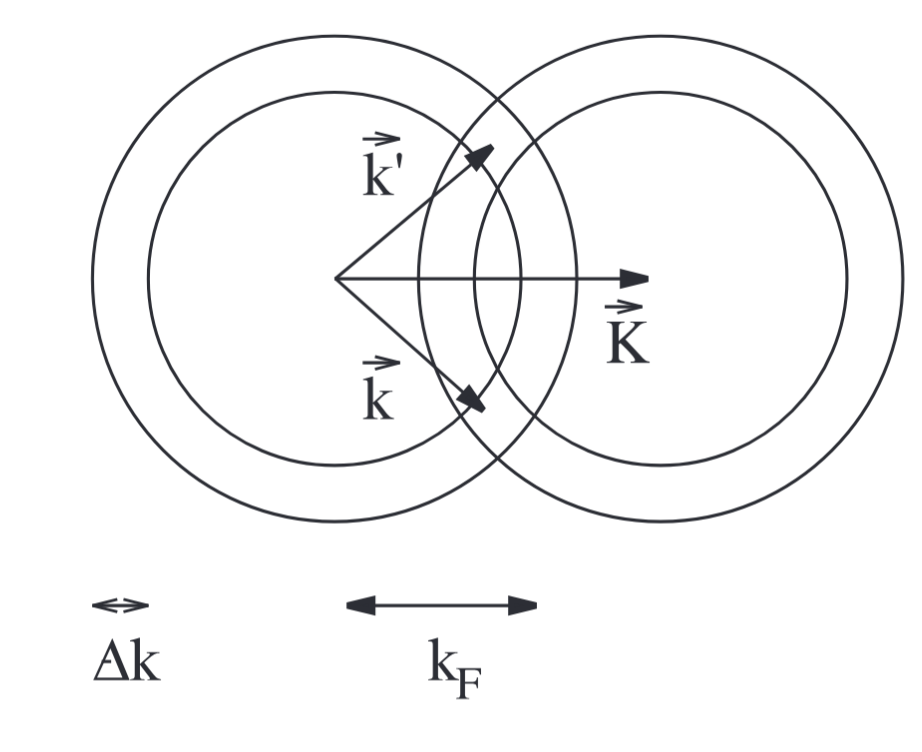
\includegraphics[width=0.4\textwidth]{images/s_wave.png}
    \caption{Erlaubte $(\vk, \vk')$ Zustände zur Bildung von Cooper-Paaren bei isotroper Dispersion. Beide Kreisringe haben den Radius $\vec{k}_\text{F}$ mit Dicke $\Delta \vk = \hbar \omega_\text{D}$ und der Überlapp beider Kreisringe gibt die erlaubten Zustände an. Für $\vec{K} \neq 0$ ist dies nur ein kleiner Teil des Kreisringes, für $\vec{K} = 0$ allerdings der gesamte Ring~\cite{czycholl_theoretische_2017}.}
    \label{fig:s_wave}
\end{figure}

Zusätzlich wird eine konstante negative Wechselwirkung $V_{\vk, \vk'} = -V$ über alle erlaubten Zustände angenommen, sodass der klassische BCS-Hamiltonian die Form
\begin{align}
    \oH_{\text{BCS}} = \sum_{\vk} \epsilon_\vk \ofed{\vk, \sigma} \ofe{\vk, \sigma} - V \sum_{\vk, \vk'}\ofed{\vk', \up} \ofed{-\vk', \down} \ofe{-\vk, \down} \ofe{\vk, \up} \Theta(\hbar \omega_D - \abs{\epsilon_\vk}) \Theta(\hbar \omega_D - \abs{\epsilon_{\vk'}})
    \label{eq:BCS}
\end{align}
mit der Heaviside-Funktion $\Theta(x)$ annimmt.

\subsection{Limitierung der BCS-Theorie}
Die BCS-Theorie kann als mikroskopische Theorie der Supraleitung die Eigenschaften konventionelle Supraleiter wie z. B. Aluminium, Blei oder Quecksilber gut beschreiben~\cite{webb_superconductivity_2015}. 
Für unkonventionelle (Hochtemperatur-) Supraleiter, wie z.B. Yttrium-Barium-Kupferoxid (YBCO) aus der Familie der Cuprate scheint der grundlegende Mechanismus der Supraleitung jedoch ein anderer zu sein. 
Die Bildung von Cooper-Paaren ist zwar auch hier die Grundlage für die Ausbildung einer supraleitenden Phase, jedoch ist die Ursache der attraktiven Wechselwirkung nicht unbedingt phononübermittelt, sondern kann z.B. auch mit Spin-Fluktuationen zusammenhängen~\cite{cao_unconventional_2018,czycholl_theoretische_2017}.
Unter diesem Aspekt ist es möglich, dass also für andere, unkonventionelle Supraleiter die in der BCS-Theorie getroffenen Annahmen für Singulett-Kopplung und einer isotropen, konstanten Wechselwirkung nicht zustimmen, weshalb in einer über der BCS-Theorie hinaus gehenden Supraleitungstheorie auch andere Kopplungsformen zugelassen werden. \\
Diese werden in der Literatur als ($s$, $p$, $d$, $f$, \dots)-wave bezeichnet, benannt nach der zugrundliegenden Symmetrie des Ordnungsparameters $\Delta(\vk)$~\cite{sigrist_phenomenological_1991}. 
Für $s$-wave ist der Ordnungsparameter isotrop, das ist also genau der Fall der durch die BCS-Theorie beschrieben wird\footnote{Ordnungsparameter, die die Symmetrie des zugrundliegenden Gitters besitzen, werden \glqq extended $s$-wave \grqq genannt. Dieser Fall wird allerdings nicht durch die BCS-Theorie beschrieben.}.